\subsection{Extraction des caractéristiques}

Afin de pouvoir utiliser un réseau de neurones pour apprendre à reconnaitre les chiffres, il était nécessaire au préalable d'extraire des caractéristiques des données de tracés fournies.

\subsubsection{Données positionnelles} Pour les données positionnelles\footnote{Les coordonnées correspondent à des grilles de $5 \times 3$, $5 \times 4$ et $7 \times 5$,} trois types de caractéristique ont été extraites.

\paragraph{L'image du tracé} L'image de tracé est reconstruite en créant une matrice de la taille de la grille des données d'entrées et de compter le nombre de fois qu'un point apparait à une coordonnée. Chaque cellule peut être considérée comme un pixel plus ou moins « lumineux ». Pour le réseaux de neurones la matrice est cependant fournit sous forme de vecteur.

\hspace{-4ex}\begin{minipage}{0.2\linewidth}
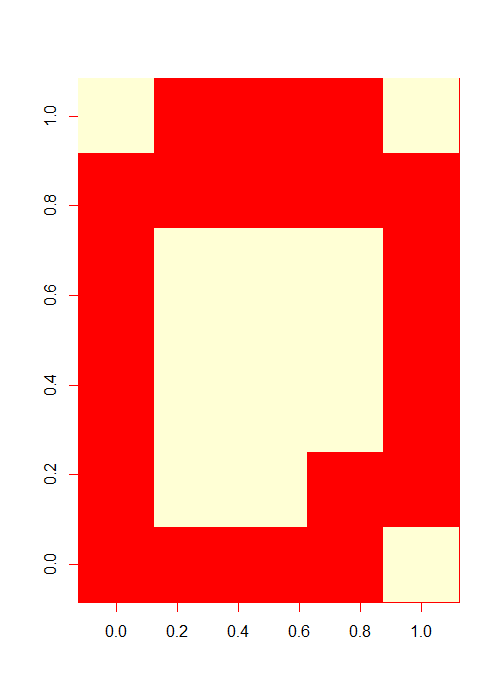
\includegraphics[width = \textwidth]{Figures/data0}
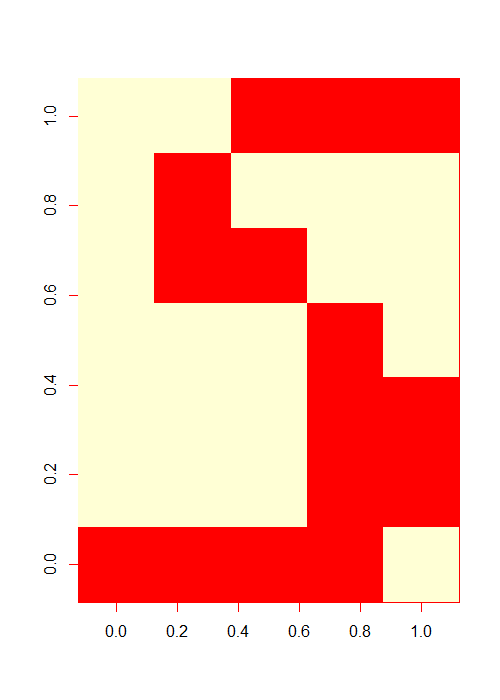
\includegraphics[width = \textwidth]{Figures/data5}
\end{minipage}
\begin{minipage}{0.2\linewidth}
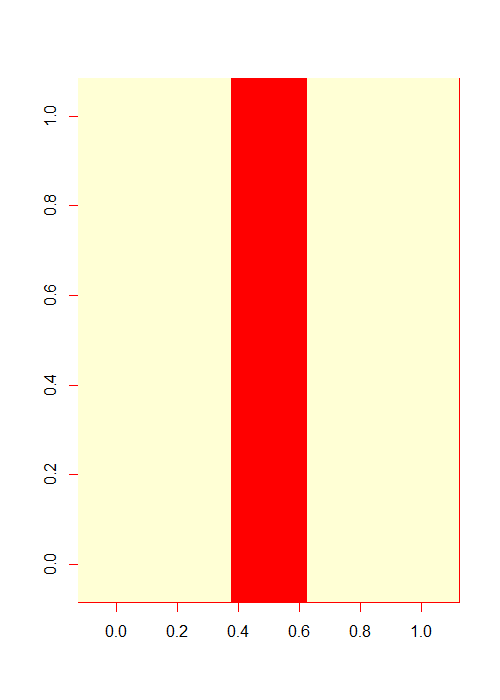
\includegraphics[width = \textwidth]{Figures/data1}
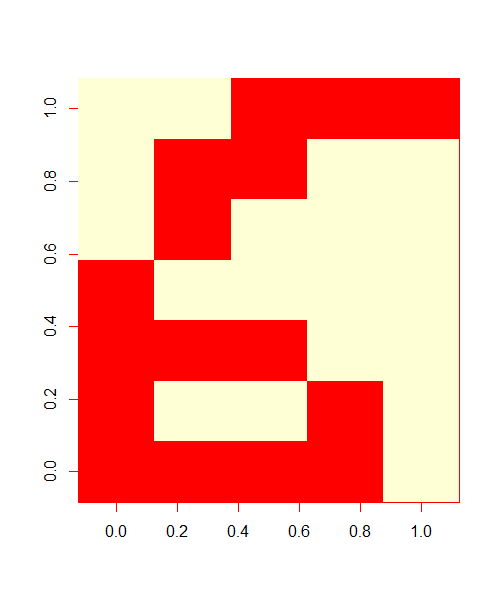
\includegraphics[width = \textwidth]{Figures/data6}
\end{minipage}
\begin{minipage}{0.2\linewidth}
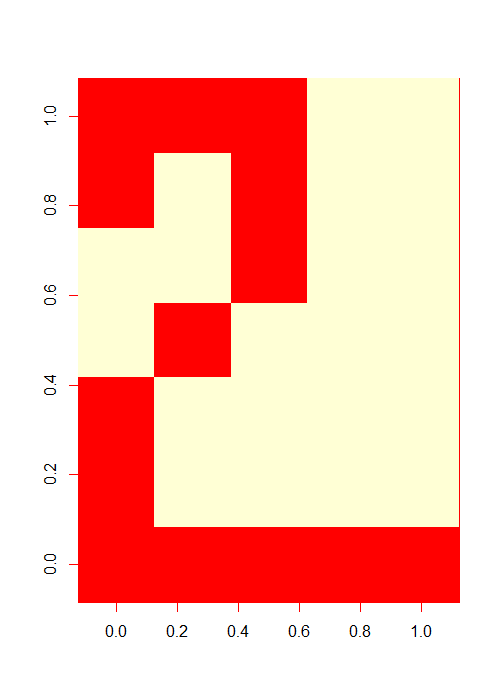
\includegraphics[width = \textwidth]{Figures/data2}
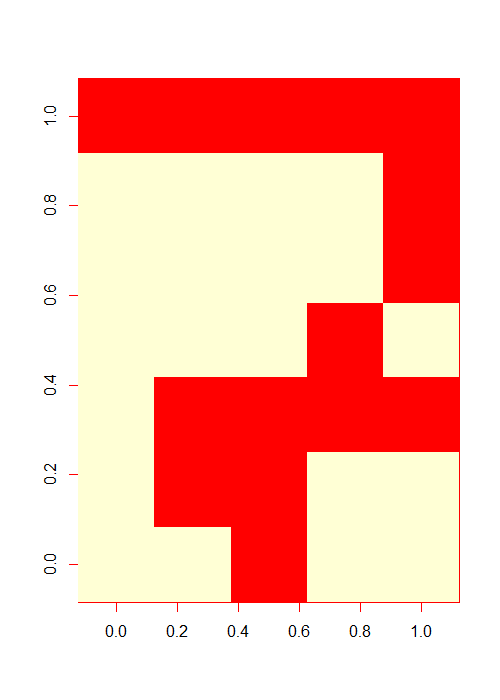
\includegraphics[width = \textwidth]{Figures/data7}
\end{minipage}
\begin{minipage}{0.2\linewidth}
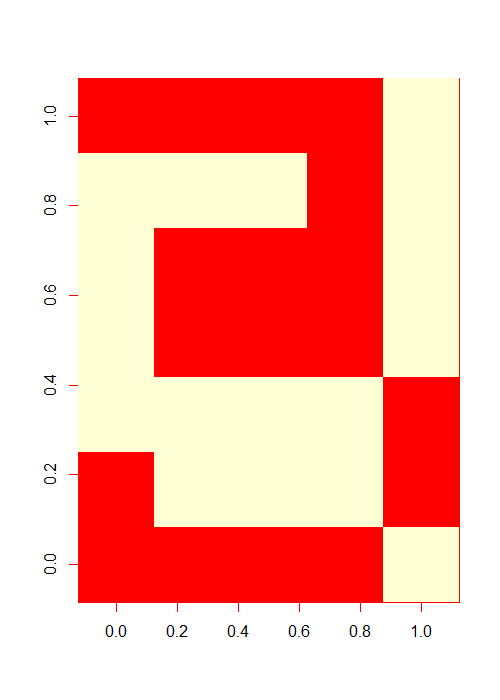
\includegraphics[width = \textwidth]{Figures/data3}
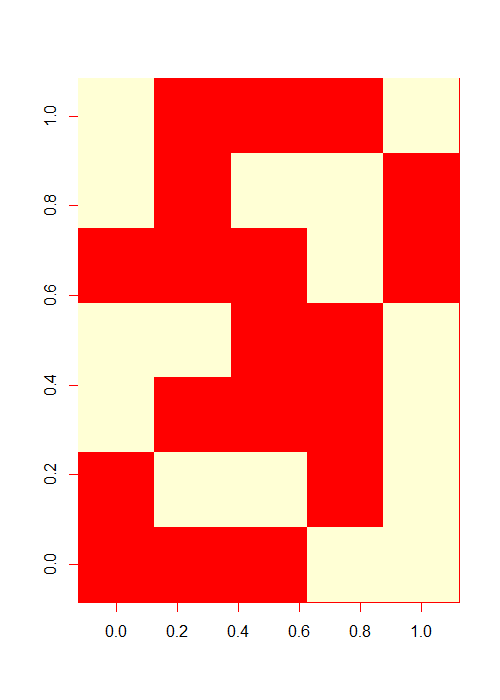
\includegraphics[width = \textwidth]{Figures/data8}
\end{minipage}
\begin{minipage}{0.2\linewidth}
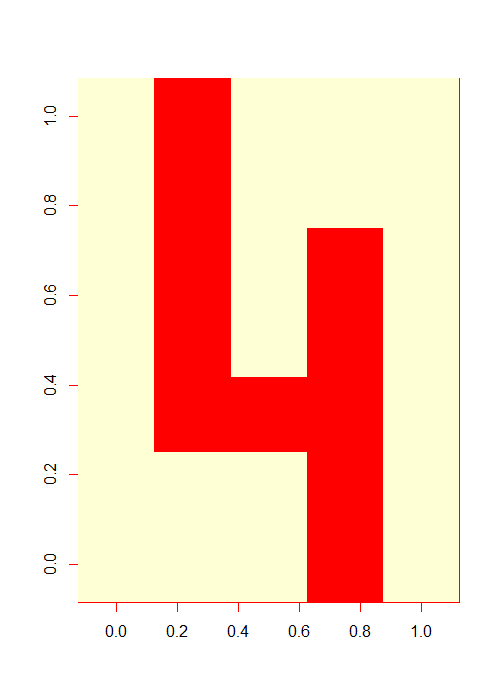
\includegraphics[width = \textwidth]{Figures/data4}
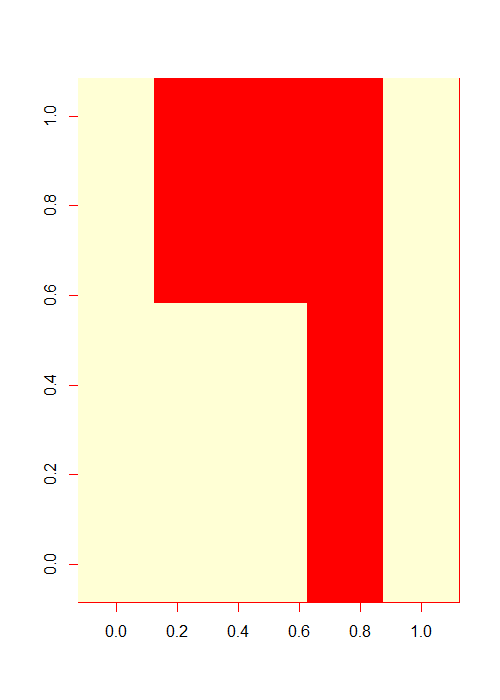
\includegraphics[width = \textwidth]{Figures/data9}
\end{minipage}




\paragraph{Les projections sur les axes} Une fois l'image reconstruite une projection sur l'axe $X$ et $Y$ sont effectuées, ce qui fournit deux vecteurs de caractéristiques supplémentaires.
\paragraph{Couverture de l'image} Sur chaque début et fin de ligne ou colonne des sondes récupèrent le premier pixel allumé à partir du bord où elles sont parties. L'ensemble de ces informations sont concaténées dans un vecteur et fournies au réseau de neurones.


\subsubsection{Données vectorielles} Ces données ont été traitées peu de temps et seulement deux vecteurs de caractéristiques ont été extraits.

\paragraph{L'occurrence des orientations de tracé} À l'instar de l'image du tracé,  le nombre des différentes orientations prises lors du tracés est mémorisé et stocké dans un vecteur\footnote{Par exemple : trois fois vers le bas, une fois à gauche...}.
\paragraph{L'occurrence des variations} Il s'agit d'un vecteur qui contient le nombre de fois que le tracé a changé de direction et avec quel importance. Par exemple un « $1$ » aura souvent 0\degre de variation tandis qu'un « $6$ » aura souvent des variations du tracé entre 10\degre et 20\degre.


\paragraph{} Les caractéristiques extraites sont ensuite données au réseau de neurones pour l'entrainement.
\subsection{Méthodologie}

\subsection{Résultats}

